
\section{Gridworld [15 pts]}

Consider the following grid environment. Starting from any unshaded square, you can move up, down, left, or right. Actions are deterministic and always succeed (e.g. going left from state 16 goes to state 15) unless they will cause the agent to run into a wall. The thicker edges indicate walls, and attempting to move in the direction of a wall results in staying in the same square (e.g. going in any direction other than left from state 16 stays in 16). Taking any action from the green target square (no. 12) earns a reward of $r_g$ (so $r(12, a)$ = $r_g$ $\forall a$) and ends the episode . Taking any action from the red square of death (no. 5) earns a reward of $r_r$ (so $r(5, a)$ = $r_r$ $\forall a$) and ends the episode. Otherwise, from every other square, taking any action is associated with a reward $r_s \in \{-1, 0, +1\}$ (even if the action results in the agent staying in the same square). Assume the discount factor $\gamma = 1$, $r_g = +5$, and $r_r = -5$ unless otherwise specified.

\begin{figure}[h]
  \centering
    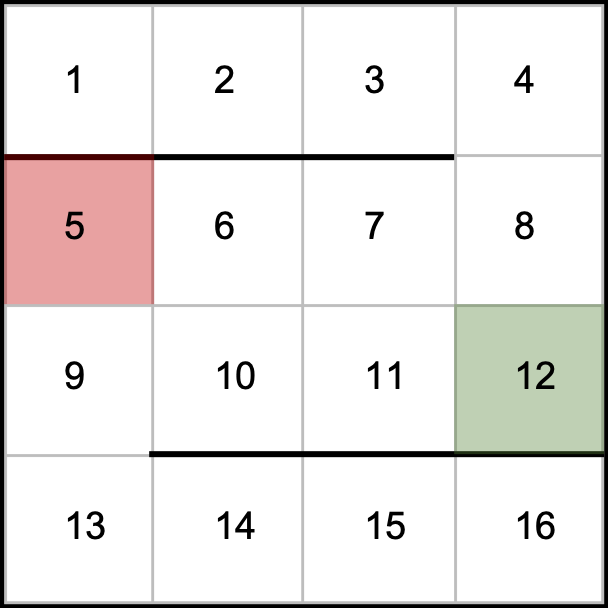
\includegraphics[width=0.3\textwidth]{tex/grid.png}
  	\label{fig:grid}
\end{figure}

\begin{enumerate}[label=(\alph*)]
\item (3pts) Define the value of $r_s$ that would cause the optimal policy to return the shortest path to the green target square (no. 12). Using this $r_s$, find the optimal value for each square.

\textbf{Answer:}

\begin{equation}
r_s = -1
\end{equation}

\begin{equation}
\begin{bmatrix}
0 & 1 & 2 & 3 \\
-5& 2 & 3 & 4 \\
2 & 3 & 4 & 5 \\
1 & 0& -1& -2
\end{bmatrix}
\end{equation}

\item (3pts) Lets refer to the value function derived in (a) as $V^{\pi_g}_{old}$ and the policy as $\pi_g$. Suppose we are now in a new gridworld where all the rewards ($r_s$, $r_g$, and $r_r$) have $+2$ added to them. Consider still following $\pi_g$ of the original gridworld, what will the new values $V^{\pi_g}_{new}$ be in this second gridworld?

\textbf{Answer:}

\begin{equation}
\begin{bmatrix}
12 & 11 & 10 & 9 \\
-3 & 10 & 9  & 8 \\
10 & 9  & 8  & 7 \\
11 & 12 & 13 & 14
\end{bmatrix}
\end{equation}

\item (3pts) Consider a general MDP with rewards, and transitions. Consider a discount factor of $\gamma$. For this case assume that the horizon is infinite (so there is no termination). A policy $\pi$ in this MDP induces a value function $V^\pi$ (lets refer to this as $V^\pi_{old}$). Now suppose we have a new MDP where the only difference is that all rewards have a constant $c$ added to them. Can you come up with an expression for the new value function $V^\pi_{new}$ induced by $\pi$ in this second MDP in terms of $V^\pi_{old}$, $c$, and $\gamma$?

\textbf{Answer:}

\begin{equation}
\begin{split}
V^\pi_{old}(s) & = \Ex_{\pi}[\sum_{t=0}^{\infty} \gamma^{t}r_t|s_0=s] \\
V^\pi_{new}(s) & = \Ex_{\pi}[\sum_{t=0}^{\infty}\gamma^{t}(r_t + c)|s_0=s] \\
               & = \Ex_{\pi}[\sum_{t=0}^{\infty}\gamma^{t}r_t|s_0=s] + c\sum_{t=0}^{\infty}\gamma^{t} \\
               & = V^\pi_{old}(s) + \frac{c}{1-\gamma}
\end{split}
\end{equation}



\item (2pts) Lets go back to our gridworld from (a) with the default values for $r_g$, $r_r$, $\gamma$ and with the value you specified for $r_s$. Suppose we now derived a second gridworld by adding a constant $c$ to all rewards ($r_s$, $r_g$, and $r_r$) such that $r_s = +2$. How does the optimal policy change (Just give a one or two sentence description)? What do the values of the unshaded squares become?

\item (2pts) Now take the second gridworld from part (d) and change $\gamma$ such that $0 < \gamma < 1$. Can the optimal policy change and does it depend on your choice of gamma? (A brief description is sufficient, no formal proof or mathematical analysis required).

\item (2pts) Lets go back to our gridworld from (a) with the default values for $r_g$, $r_r$, $\gamma$ and with the value you specified for $r_s$. In this gridworld, our optimal policy from any unshaded square never terminates in the red square. Now suppose $r_s$ can take on any real, non-infinite value and is not restricted to $\{+1, 0, -1\}$ anymore. Give a value of $r_s$ such that there are unshaded squares starting from which following the optimal policy results in termination in the red square.


\end{enumerate}
